% Условная компиляция для самостоятельной работы
\ifdefined\mainfile
    % Если это часть основного файла, не добавляем начало и конец документа
\else
    \documentclass[12pt, a4paper]{report}
    \usepackage{/Users/vladbelousov/Desktop/Semestr_4-FP-NSU/Настройка/library}
    \usepackage[utf8]{inputenc} % Подключение поддержки UTF-8
    \begin{document}
\fi

%%-------------------------------%%

Опты Юнга (продолжение). Идея осуществить интерференцию от различных частей волнового фронта (поделить фронт волны)

\begin{center}
    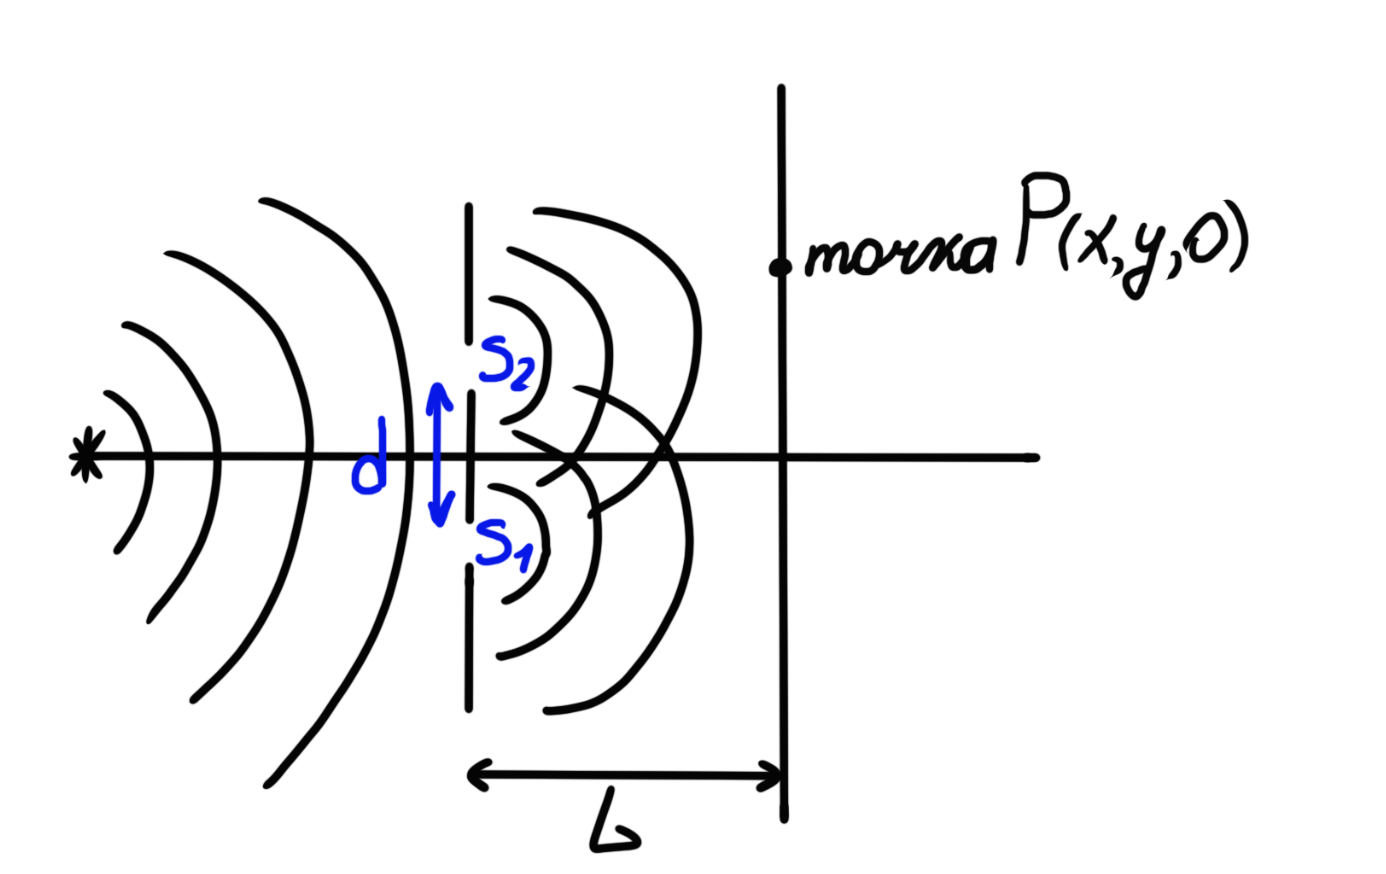
\includegraphics[width=0.5\textwidth]{/Users/vladbelousov/Desktop/Semestr_4-FP-NSU/ЭиО/Лекции_по_дням/image/105.png}
\end{center}  

\[ \vec{E }  _1 = |E_0 ^{\perp }  | \frac{L}{r_1 } e^{i k r_1 - i \omega_0 t + i \varphi_1 (t)} \vec{e } _3   , \quad  \varphi_1 (t ) = \varphi_s \left(  t - \frac{r_1}{c}  \right)\] 
\[ \vec{E }  _2 = |E_0 ^{\perp }  | \frac{L}{r_2 } e^{i k r_2 - i \omega_0 t + i \varphi_2 (t)}\vec{e } _3  , \quad  \varphi_2 (t ) = \varphi_s \left(  t - \frac{r_2}{c}  \right)\] 

\[ I^{\perp } = I_1 ^{\perp } + I_2 ^{\perp } +I_{12} ^{\perp } =\frac{1}{2 }  \frac{|E_0  ^{\perp }  | ^2 L ^2 }{r_1 ^2 } + \frac{1}{2 }  \frac{|E_0 ^{\perp } |L ^2 }{r_2 ^2 } + \frac{|E_0 ^{\perp } | ^2 L ^2 }{ r_1 r_2 } \underbrace{<\cos (k \Delta r +\delta \varphi(t ))>  }_{\text{усреднение по } \tau_0 \text{ - прибора}  }      \] 
, где \( \displaystyle \delta(t ) = \varphi_s \left(  t - \frac{r_1 }{c} \right) - \varphi_s \left( t - \frac{r_2 }{c}  \right) = \varphi_s(t ' ) - \varphi_s \left( t ' + \frac{\Delta r }{c }  \right) \) 

Если \( \displaystyle  \frac{\Delta r }{ c } < \tau_{\text{ког} } =\frac{1}{\gamma}    \), то \( \delta \varphi (t ) \approx 0 \)  и интерференционная картина зависит от \( \Delta r \) и видна. 

Если \( \displaystyle  \frac{\Delta r }{c } > \tau _{\text{ког} } = \frac{1}{\gamma }    \), то \( \displaystyle  \delta \varphi (t )  \) - случайная величина и \( <\cos ( k \Delta r + \delta \varphi (t ))> = 0 \Rightarrow \)  интерференционная картина  не наблюдается. 

\( \Delta r  \)  при котором интерференционная картина исчезает называется \textbf{продольная длина когерентности}:

\[ l_{\parallel } = c \tau_{\text{ког} } = \frac{c}{\gamma } =\left[ \Delta \omega \Delta t \sim  \pi \Rightarrow \Delta t = \frac{\pi}{\Delta \omega } = \frac{\pi}{\gamma}   \right] = \frac{c \pi } {\Delta \omega } = \frac{ c \pi \lambda ^2 }{ 2 \pi c \Delta \lambda } = \frac{\lambda ^2 }{2 \Delta \lambda }       \] 
\[ \left( \omega = \frac{ 2 \pi c }{\lambda } \Rightarrow |\Delta \omega     |  = \frac{ 2 \pi c }{\lambda ^2 } |\Delta \lambda | \right) \] 


Для свечения разряженного газа \( \displaystyle  l_{\parallel } = \frac{3 \cdot 10^{ 10 }  }{10^{9 } } = 30 \text{ см}    \) (За счет столкновений атомов \( l_{\parallel}  \) снижается до \( \sim f \text{ см}  \))

\[ \Delta r= \frac{x d }{ L } \sim 1 \text{ см }  \quad  x  = 1 \cdot \frac{ 100}{ 0,1 }  \sim 10^{3 }  \text{ см}  \] 

\textbf{Опыт Юнга (качественный анализ)}: 

Пусть спектр источника - прямоугольный (приближение). 

\begin{center}
    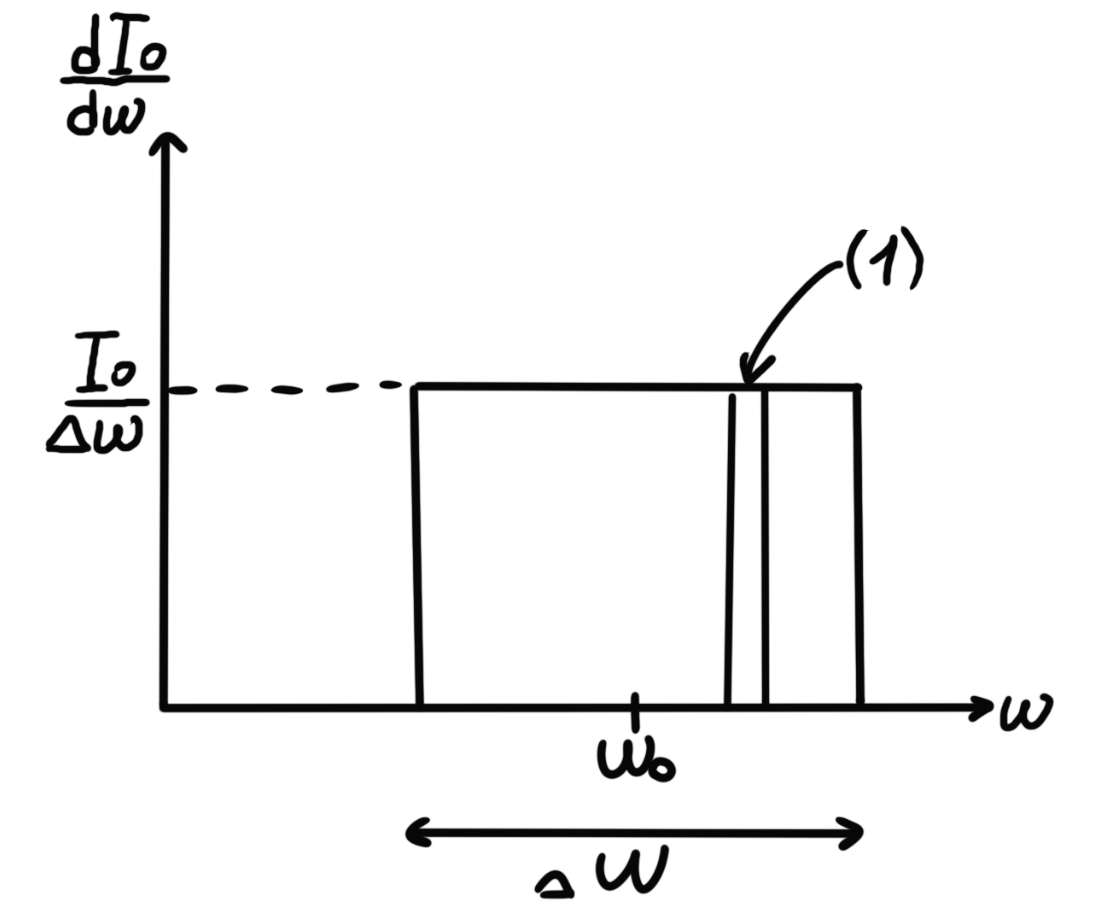
\includegraphics[width=0.4\textwidth]{/Users/vladbelousov/Desktop/Semestr_4-FP-NSU/ЭиО/Лекции_по_дням/image/106.png}
\end{center}  
\[ \text{(1): ширина } d \omega \text{ такая, чтобы } l_{\parallel } ' = \frac{cT }{d \omega } \gg \Delta r \text{ - разность хода в экспоненте}     \] 

\[ d I_0 = d I_1 = d I_2 ( \text{т.к } L \gg x,d,y  ) \] 

\[ dI = d I_1 + d I_2 + \sqrt{d I_1 d I_2 } 2 \cos (k \Delta r ) = 2 d I_0 \left( 1 + \cos \left( \frac{\omega}{c }  \Delta r \right) \right) \] 

\[ I = \int d I = \int_{\omega_0- \frac{\Delta \omega }{2 } }^{\omega_0+ \frac{\Delta \omega }{2 }  } 2 \frac{d I_0 }{d \omega } \left( 1 + \cos \left( \frac{ \omega }{c } \Delta r   \right) \right) d \omega = 2 \frac{ I_0 }{\Delta \omega } \left( \Delta \omega + \frac{ \sin \left( \frac{\omega}{c }  \Delta r \right)}{\frac{\Delta r}{c} } \bigg | ^{\omega_0 + \frac{\Delta \omega }{2 }  }_{\omega_0 - \frac{\Delta \omega }{2} }   \right) = \] 
\[= 2 I_0 \left( 1+\frac{  2 \cos \left( \frac{\Delta r}{c} \omega_0  \right) \sin \left( \frac{\Delta r}{c } \frac{\Delta \omega }{2 }   \right) }{\frac{ \Delta r \Delta \omega}{ 2 c } } \right)  = 2 I_0 \bigg( 1 + \underbrace{\mathrm{sinc }  \left( \frac{\Delta r }{c } \Delta \omega   \right)}_{\text{огибающая} } \underbrace{\cos \left( \frac{\Delta r }{c } \omega_0  \right)}_{\text{наполнение} }  \bigg)\] 

\[  \text{Видность: } I_{\max  } = 2 I_0 (1 + |\mathrm{sinc }   |) , \quad  I_{ \min  } = 2 I_0 (1 - |\mathrm{sinc}  |) \]
\[ V = \frac{2 I_0 2 |\mathrm{sinc}  |}{4 I_0 } = \left\lvert \mathrm{sinc }  \left( \frac{\Delta \omega \Delta r }{2 c }  \right)  \right\rvert  \]  

\begin{center}
    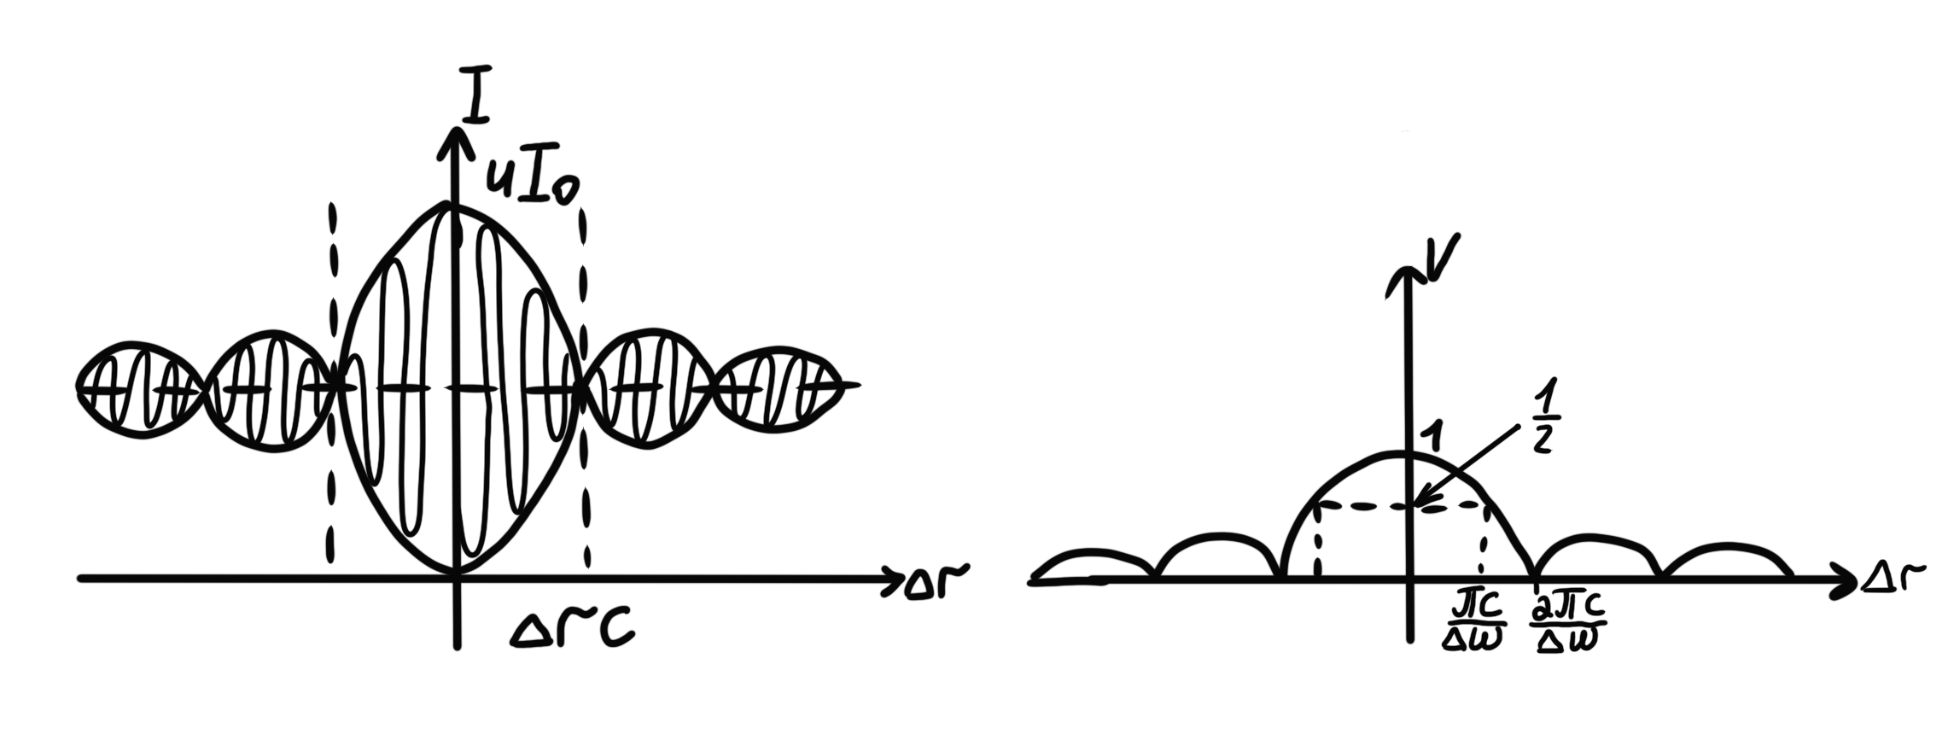
\includegraphics[width=0.8\textwidth]{/Users/vladbelousov/Desktop/Semestr_4-FP-NSU/ЭиО/Лекции_по_дням/image/107.png}
\end{center}  

Если \( \Delta r > \displaystyle  \frac{ \pi c }{\Delta \omega }   \) - картина интерференции исчезает; 

\vspace{10pt}

Если \( \displaystyle  \Delta r < \frac{\pi c }{\Delta \omega }  \) - картина видна.

\[ \Delta r_m = \frac{ x_m d }{L } = m \lambda \quad  (\text{условие максимума интенсивности} )  \] 
\[ \frac{\Delta r_m \omega_0 }{c } = 2 \pi m   \] 
\[ \frac{\Delta r_m }{\lambda }     = m   \] 
\[ \Delta r_m = \lambda m  \] 
\[ x_m = \frac{L }{d} m \lambda   \] 
\[ x_{m+1 } - x_m = \Delta x_m = \frac{\lambda L }{d}  \] 

Размер интерференционной картины \( \displaystyle  l_{\parallel} = \Delta r = \frac{x_{ \max  } d }{L }   \) 

\[ \Rightarrow  x_{ \max  } = \frac{L}{d } l_{ \parallel} = \frac{L}{d }  \frac{\pi c }{\Delta \omega }    \] 
\[ 2 x_{ \max  } = \frac{L}{d }  \frac{ 2 \pi c }{\Delta \omega } , \text{ число полос: }    \] 
\[ \frac{x _{ \max  } }{\Delta x_m }= \frac{d}{ \lambda L } \frac{L }{d} \frac{ 2 \pi c \omega_0 }{\Delta \omega \omega_0} = \frac{\omega_0}{\Delta \omega}      \] 

Влияние размера источника на интерференционную картину: 

\begin{center}
    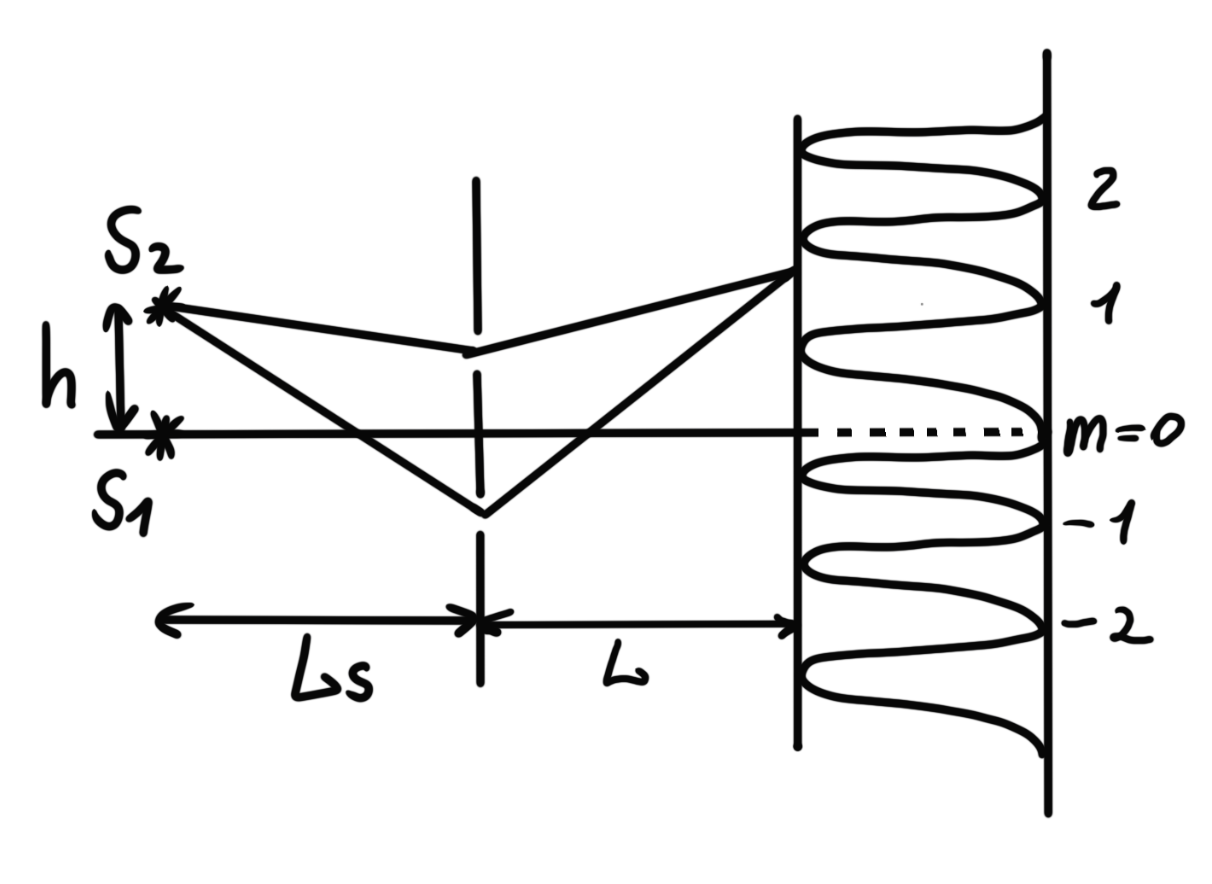
\includegraphics[width=0.4\textwidth]{/Users/vladbelousov/Desktop/Semestr_4-FP-NSU/ЭиО/Лекции_по_дням/image/108.png}
\end{center} 

\[ \Delta r (\text{смещенного на } h \text{ источника} ) = r_1 ' + r_1 - r_2 -r_2 ' ; \quad  r_1 ' - r_2 ' = \frac{h}{L_s } d \] 
\[ d \alpha \approx \frac{h}{L_s} d = \Delta_1 ;\quad  r_1 -r_2 = \frac{x}{L }  d = \Delta_2  \] 
\[ \Delta r_m = \Delta_1 + \Delta_2 = \frac{h}{L_s } d + \frac{x}{L }  d = m' \lambda   \]
, где \( m '  \) - порядок второго источника. 

\[ \frac{h}{L_s } + \frac{x_0 }{L } = 0   \] 

Первый раз когда исчезнет (при увеличении \( h \)) интерференционная картина:

\[ \displaystyle  \left( \frac{h^* }{L_s } + \frac{0}{L }   \right)d = \frac{\lambda}{2 }  , \quad  h^* = \frac{\lambda L_s}{2d}  \] 

но потом периодически появляется и исчезает, так как интерференционные картины двух источников,то синфазны, то наблюдаются в противофазе.

Каждый участок источника является скоплением случайно излучающих атомов и не интерферирует с соседним участком \( \Rightarrow \)  складываем интерференционные картины от разных участков.

\begin{center}
    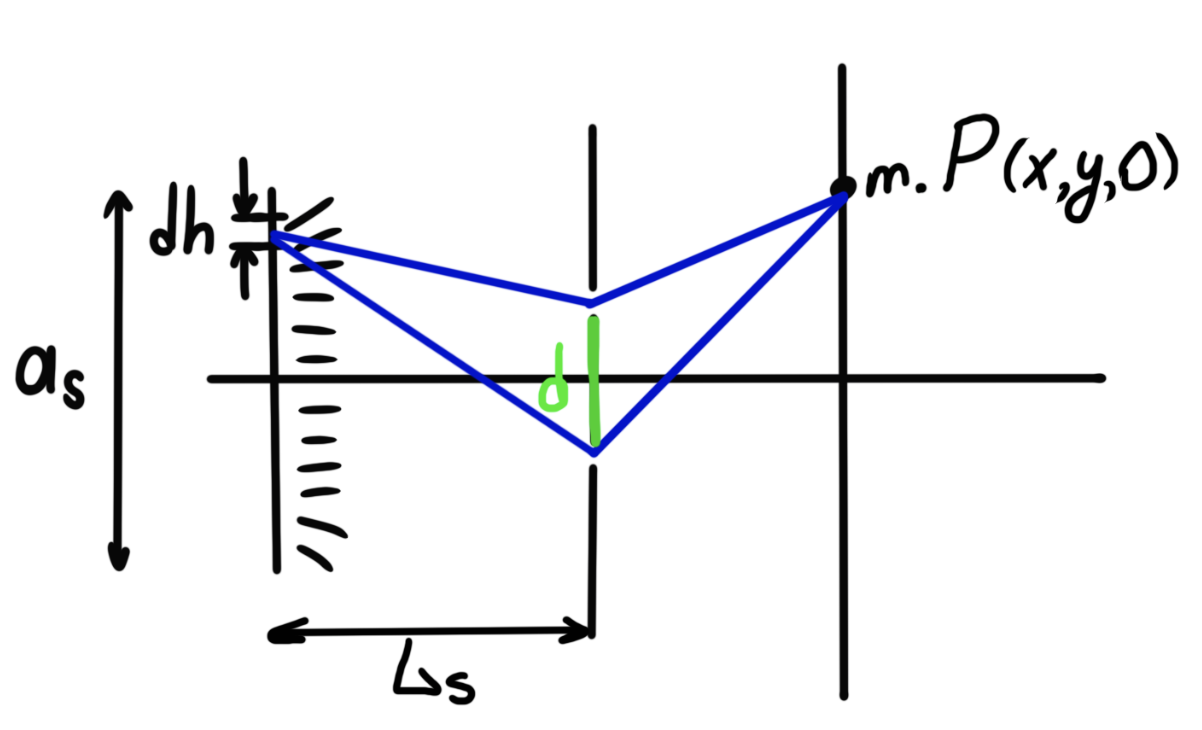
\includegraphics[width=0.5\textwidth]{/Users/vladbelousov/Desktop/Semestr_4-FP-NSU/ЭиО/Лекции_по_дням/image/109.png}
\end{center}  

Рассмотрим только центр интерференционной картины, где 
\[  \displaystyle  \frac{\Delta r \Delta \omega }{2 c } \ll \pi \quad  ( \Delta r \ll l_{ \parallel} ) \] 

\[ d I_0 = d I_1 = d I_2 \quad  L_s , \text{ }  L \gg d, h, x ,y \]
\[ d I_0 = \frac{I_0}{a_s}  \]  

\begin{center}
    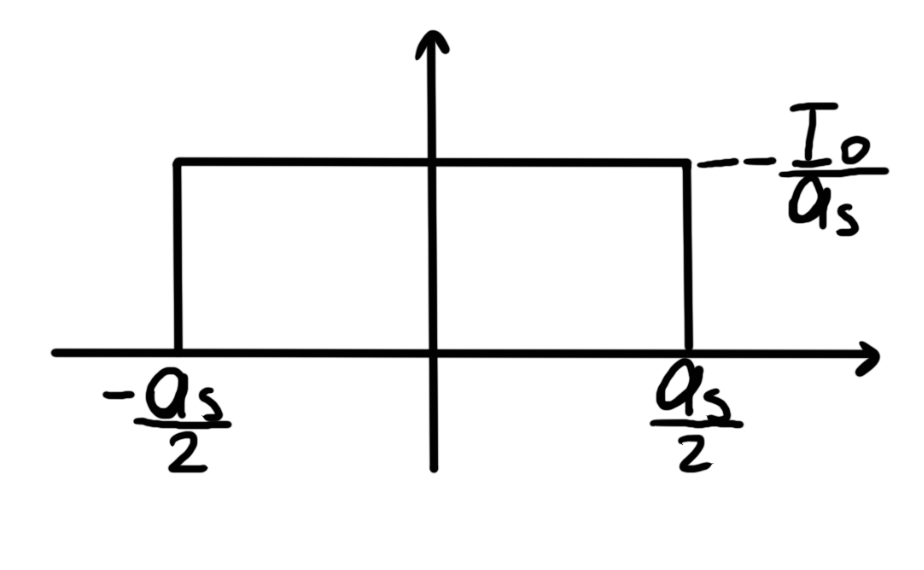
\includegraphics[width=0.5\textwidth]{/Users/vladbelousov/Desktop/Semestr_4-FP-NSU/ЭиО/Лекции_по_дням/image/110.png}
\end{center} 

\[ d I = 2 d I_0 (1 + \cos \omega_0 k \Delta r ) = \frac{2 d I_0 }{dh      } dh \left( 1 + \cos \left[ k d \left( \frac{x}{L }  + \frac{h}{L_s}  \right) \right] \right)\text{ }  \bigg |\cdot \int _{-\frac{a_s}{2 }  } ^{\frac{a_s}{2 } }     \] 
\[ I = \frac{2 I_0 }{a_s } \left( a_s +\frac{\sin \left( kd \left( \frac{x}{L } + \frac{h}{L_s }  \right) \right)}{k \frac{d}{L_s} }\bigg |_{-\frac{a_s}{2} }^{\frac{a_s}{2} }    \right)   \] 
%%-------------------------------%%

% Закрытие документа, если файл компилируется отдельно
\ifdefined\mainfile
    % Если это основной файл, не нужно заканчивать документ
\else
    \end{document}
\fi

